\documentclass[nooutcomes, noauthor]{ximera}


\graphicspath{
  {./}
  {1-1QuantitativeReasoning/}
  {1-2RelationsAndGraphs/}
  {1-3ChangingInTandem/}
  {2-1LinearEquations/}
  {2-2LinearModeling/}
  {2-3ExponentialModeling/}
  {3-1WhatIsAFunction/}
  {3-2FunctionProperties/}
  {3-3AverageRatesOfChange/}
  {4-1BuildingNewFunctions/}
  {4-2Polynomials/}
  {5-1RationalFunctions/}
   {5-2ExponentialFunctions/}
  {6-1Domain/}
  {6-2Range/}
  {6-3CompositionOfFunctions/}
  {7-1ZerosOfFunctions/}
  {7-XZerosOfPolynomials/}
  {7-2ZerosOfFamousFunctions/}
  {8-0Review/}
  {8-1FunctionTransformations/}
  {8-2SolvingInequalities/}
  {8-3FunctionTransformationsProject/}
  {9-1RightTriangleTrig/}
  {9-2TheUnitCircle/}
  {9-3TrigIdentities/}
  {10-1UnitCircleToFunctionGraph/}
  {10-2TrigFunctions/}
  {10-3SomeApplicationsOfTrig/}
  {11-1InverseFunctionsRevisited/}
  {11-2Logarithms/}
  {11-3InverseTrig/}
  {12-1SystemsOfEquations/}
  {12-2NonlinearSystems/}
  {12-3ApplicationsOfSystems/}
  {13-1SecantLinesRevisited/}
  {13-2Functions-TheBigPicture/}
  {14-1DisplacementVsDistance/}
  {1-1QuantitativeReasoning/exercises/}
  {1-2RelationsAndGraphs/exercises/}
  {../1-3ChangingInTandem/exercises/}
  {../2-1LinearEquations/exercises/}
  {../2-2LinearModeling/exercises/}
  {../2-3ExponentialModeling/exercises/}
  {../3-1WhatIsAFunction/exercises/}
  {../3-2FunctionProperties/exercises/}
  {../3-3AverageRatesOfChange/exercises/}
  {../5-2ExponentialFunctions/exercises/}
  {../4-1BuildingNewFunctions/exercises/}
  {../4-2Polynomials/exercises/}
  {../5-1RationalFunctions/exercises/}
  {../6-1Domain/exercises/}
  {../6-2Range/exercises/}
  {../6-3CompositionOfFunctions/exercises/}
  {../7-1ZerosOfFunctions/exercises/}
  {../7-XZerosOfPolynomials/exercises/}
  {../7-2ZerosOfFamousFunctions/exercises/}
  {../8-1FunctionTransformations/exercises/}
  {../12-1SystemsOfEquations/exercises/}
  {../8-3FunctionTransformationsProject/exercises/}
  {../8-0Review/exercises/}
  {../8-2SolvingInequalities/exercises/}
  {../8-3FunctionTransformationsProject/exercises/}
  {../9-1RightTriangleTrig/exercises/}
  {../9-2TheUnitCircle/exercises/}
  {../9-3TrigIdentities/exercises/}
  {../10-1UnitCircleToFunctionGraph/exercises/}
  {../10-2TrigFunctions/exercises/}
  {../10-3SomeApplicationsOfTrig/exercises/}
  {../11-1InverseFunctionsRevisited/exercises/}
  {../11-2Logarithms/exercises/}
  {../11-3InverseTrig/exercises/}
  {../12-1SystemsOfEquations/exercises/}
  {../12-2NonlinearSystems/exercises/}
  {../12-3ApplicationsOfSystems/exercises/}
  {../13-1SecantLinesRevisited/exercises/}
  {../13-2Functions-TheBigPicture/exercises/}
  {../14-1DisplacementVsDistance/exercises/}
}

\DeclareGraphicsExtensions{.pdf,.png,.jpg,.eps}

\newcommand{\mooculus}{\textsf{\textbf{MOOC}\textnormal{\textsf{ULUS}}}}

\usepackage[makeroom]{cancel} %% for strike outs

\ifxake
\else
\usepackage[most]{tcolorbox}
\fi


%\typeout{************************************************}
%\typeout{New Environments}
%\typeout{************************************************}

%% to fix for web can be removed when deployed offically with ximera2
\let\image\relax\let\endimage\relax
\NewEnviron{image}{% 
  \begin{center}\BODY\end{center}% center
}



\NewEnviron{folder}{
      \addcontentsline{toc}{section}{\textbf{\BODY}}
}

\ifxake
\let\summary\relax
\let\endsummary\relax
\newtheorem*{summary}{Summary}
\newtheorem*{callout}{Callout}
\newtheorem*{overview}{Overview}
\newtheorem*{objectives}{Objectives}
\newtheorem*{motivatingQuestions}{Motivating Questions}
\newtheorem*{MM}{Metacognitive Moment}
      
%% NEEDED FOR XIMERA 2
%\ximerizedEnvironment{summary}
%\ximerizedEnvironment{callout}
%\ximerizedEnvironment{overview} 
%\ximerizedEnvironment{objectives}
%\ximerizedEnvironment{motivatingQuestions}
%\ximerizedEnvironment{MM}
\else
%% CALLOUT
\NewEnviron{callout}{
  \begin{tcolorbox}[colback=blue!5, breakable,pad at break*=1mm]
      \BODY
  \end{tcolorbox}
}
%% MOTIVATING QUESTIONS
\NewEnviron{motivatingQuestions}{
  \begin{tcolorbox}[ breakable,pad at break*=1mm]
    \textbf{\Large Motivating Questions}\hfill
    %\begin{itemize}[label=\textbullet]
      \BODY
    %\end{itemize}
  \end{tcolorbox}
}
%% OBJECTIVES
\NewEnviron{objectives}{  
    \vspace{.5in}
      %\begin{tcolorbox}[colback=orange!5, breakable,pad at break*=1mm]
    \textbf{\Large Learning Objectives}
    \begin{itemize}[label=\textbullet]
      \BODY
    \end{itemize}
    %\end{tcolorbox}
}
%% DEFINITION
\let\definition\relax
\let\enddefinition\relax
\NewEnviron{definition}{
  \begin{tcolorbox}[ breakable,pad at break*=1mm]
    \noindent\textbf{Definition}~
      \BODY
  \end{tcolorbox}
}
%% OVERVIEW
\let\overview\relax
\let\overview\relax
\NewEnviron{overview}{
  \begin{tcolorbox}[ breakable,pad at break*=1mm]
    \textbf{\Large Overview}
    %\begin{itemize}[label=\textbullet] %% breaks Xake
      \BODY
    %\end{itemize}
  \end{tcolorbox}
}
%% SUMMARY
\let\summary\relax
\let\endsummary\relax
\NewEnviron{summary}{
  \begin{tcolorbox}[ breakable,pad at break*=1mm]
    \textbf{\Large Summary}
    %\begin{itemize}[label=\textbullet] %% breaks Xake
      \BODY
    %\end{itemize}
  \end{tcolorbox}
}
%% REMARK
\let\remark\relax
\let\endremark\relax
\NewEnviron{remark}{
  \begin{tcolorbox}[colback=green!5, breakable,pad at break*=1mm]
    \noindent\textbf{Remark}~
      \BODY
  \end{tcolorbox}
}
%% EXPLANATION
\let\explanation\relax
\let\endexplanation\relax
\NewEnviron{explanation}{
    \normalfont
    \noindent\textbf{Explanation}~
      \BODY
}
%% EXPLORATION
\let\exploration\relax
\let\endexploration\relax
\NewEnviron{exploration}{
  \begin{tcolorbox}[colback=yellow!10, breakable,pad at break*=1mm]
    \noindent\textbf{Exploration}~
      \BODY
  \end{tcolorbox}
}
%% METACOGNITIVE MOMENTS
\let\MM\relax
\let\endMM\relax
\NewEnviron{MM}{
  \begin{tcolorbox}[colback=pink!15, breakable,pad at break*=1mm]
    \noindent\textbf{Metacognitive Moment}~
      \BODY
  \end{tcolorbox}
}


\fi





%Notes on what envirnoment to use:  Example with Explanation in text; if they are supposed to answer- Problem; no answer - Exploration


%\typeout{************************************************}
%% Header and footers
%\typeout{************************************************}

\newcommand{\licenseAcknowledgement}{Licensed under Creative Commons 4.0}
\newcommand{\licenseAPC}{\renewcommand{\licenseAcknowledgement}{\textbf{Acknowledgements:} Active Prelude to Calculus (https://activecalculus.org/prelude) }}
\newcommand{\licenseSZ}{\renewcommand{\licenseAcknowledgement}{\textbf{Acknowledgements:} Stitz Zeager Open Source Mathematics (https://www.stitz-zeager.com/) }}
\newcommand{\licenseAPCSZ}{\renewcommand{\licenseAcknowledgement}{\textbf{Acknowledgements:} Active Prelude to Calculus (https://activecalculus.org/prelude) and Stitz Zeager Open Source Mathematics (https://www.stitz-zeager.com/) }}
\newcommand{\licenseORCCA}{\renewcommand{\licenseAcknowledgement}{\textbf{Acknowledgements:}Original source material, products with readable and accessible
math content, and other information freely available at pcc.edu/orcca.}}
\newcommand{\licenseY}{\renewcommand{\licenseAcknowledgement}{\textbf{Acknowledgements:} Yoshiwara Books (https://yoshiwarabooks.org/)}}
\newcommand{\licenseOS}{\renewcommand{\licenseAcknowledgement}{\textbf{Acknowledgements:} OpenStax College Algebra (https://openstax.org/details/books/college-algebra)}}
\newcommand{\licenseAPCSZCSCC}{\renewcommand{\licenseAcknowledgement}{\textbf{Acknowledgements:} Active Prelude to Calculus (https://activecalculus.org/prelude), Stitz Zeager Open Source Mathematics (https://www.stitz-zeager.com/), CSCC PreCalculus and Calculus texts (https://ximera.osu.edu/csccmathematics)}}

\ifxake\else %% do nothing on the website
\usepackage{fancyhdr}
\pagestyle{fancy}
\fancyhf{}
\fancyhead[R]{\sectionmark}
\fancyfoot[L]{\thepage}
\fancyfoot[C]{\licenseAcknowledgement}
\renewcommand{\headrulewidth}{0pt}
\renewcommand{\footrulewidth}{0pt}
\fi

%%%%%%%%%%%%%%%%



%\typeout{************************************************}
%\typeout{Table of Contents}
%\typeout{************************************************}


%% Edit this to change the font style
\newcommand{\sectionHeadStyle}{\sffamily\bfseries}


\makeatletter

%% part uses arabic numerals
\renewcommand*\thepart{\arabic{part}}


\ifxake\else
\renewcommand\chapterstyle{%
  \def\maketitle{%
    \addtocounter{titlenumber}{1}%
    \pagestyle{fancy}
    \phantomsection
    \addcontentsline{toc}{section}{\textbf{\thepart.\thetitlenumber\hspace{1em}\@title}}%
                    {\flushleft\small\sectionHeadStyle\@pretitle\par\vspace{-1.5em}}%
                    {\flushleft\LARGE\sectionHeadStyle\thepart.\thetitlenumber\hspace{1em}\@title \par }%
                    {\setcounter{problem}{0}\setcounter{sectiontitlenumber}{0}}%
                    \par}}





\renewcommand\sectionstyle{%
  \def\maketitle{%
    \addtocounter{sectiontitlenumber}{1}
    \pagestyle{fancy}
    \phantomsection
    \addcontentsline{toc}{subsection}{\thepart.\thetitlenumber.\thesectiontitlenumber\hspace{1em}\@title}%
    {\flushleft\small\sectionHeadStyle\@pretitle\par\vspace{-1.5em}}%
    {\flushleft\Large\sectionHeadStyle\thepart.\thetitlenumber.\thesectiontitlenumber\hspace{1em}\@title \par}%
    %{\setcounter{subsectiontitlenumber}{0}}%
    \par}}



\renewcommand\section{\@startsection{paragraph}{10}{\z@}%
                                     {-3.25ex\@plus -1ex \@minus -.2ex}%
                                     {1.5ex \@plus .2ex}%
                                     {\normalfont\large\sectionHeadStyle}}
\renewcommand\subsection{\@startsection{subparagraph}{10}{\z@}%
                                    {3.25ex \@plus1ex \@minus.2ex}%
                                    {-1em}%
                                    {\normalfont\normalsize\sectionHeadStyle}}

\fi

%% redefine Part
\renewcommand\part{%
   {\setcounter{titlenumber}{0}}
  \if@openright
    \cleardoublepage
  \else
    \clearpage
  \fi
  \thispagestyle{plain}%
  \if@twocolumn
    \onecolumn
    \@tempswatrue
  \else
    \@tempswafalse
  \fi
  \null\vfil
  \secdef\@part\@spart}

\def\@part[#1]#2{%
    \ifnum \c@secnumdepth >-2\relax
      \refstepcounter{part}%
      \addcontentsline{toc}{part}{\thepart\hspace{1em}#1}%
    \else
      \addcontentsline{toc}{part}{#1}%
    \fi
    \markboth{}{}%
    {\centering
     \interlinepenalty \@M
     \normalfont
     \ifnum \c@secnumdepth >-2\relax
       \huge\sffamily\bfseries \partname\nobreakspace\thepart
       \par
       \vskip 20\p@
     \fi
     \Huge \bfseries #2\par}%
    \@endpart}
\def\@spart#1{%
    {\centering
     \interlinepenalty \@M
     \normalfont
     \Huge \bfseries #1\par}%
    \@endpart}
\def\@endpart{\vfil\newpage
              \if@twoside
               \if@openright
                \null
                \thispagestyle{empty}%
                \newpage
               \fi
              \fi
              \if@tempswa
                \twocolumn
                \fi}



\makeatother





%\typeout{************************************************}
%\typeout{Stuff from Ximera}
%\typeout{************************************************}



\usepackage{array}  %% This is for typesetting long division
\setlength{\extrarowheight}{+.1cm}
\newdimen\digitwidth
\settowidth\digitwidth{9}
\def\divrule#1#2{
\noalign{\moveright#1\digitwidth
\vbox{\hrule width#2\digitwidth}}}





\newcommand{\RR}{\mathbb R}
\newcommand{\R}{\mathbb R}
\newcommand{\N}{\mathbb N}
\newcommand{\Z}{\mathbb Z}

\newcommand{\sagemath}{\textsf{SageMath}}


\def\d{\,d}
%\renewcommand{\d}{\mathop{}\!d}
\newcommand{\dd}[2][]{\frac{\d #1}{\d #2}}
\newcommand{\pp}[2][]{\frac{\partial #1}{\partial #2}}
\renewcommand{\l}{\ell}
\newcommand{\ddx}{\frac{d}{\d x}}



%\newcommand{\unit}{\,\mathrm}
\newcommand{\unit}{\mathop{}\!\mathrm}
\newcommand{\eval}[1]{\bigg[ #1 \bigg]}
\newcommand{\seq}[1]{\left( #1 \right)}
\renewcommand{\epsilon}{\varepsilon}
\renewcommand{\phi}{\varphi}


\renewcommand{\iff}{\Leftrightarrow}

\DeclareMathOperator{\arccot}{arccot}
\DeclareMathOperator{\arcsec}{arcsec}
\DeclareMathOperator{\arccsc}{arccsc}
\DeclareMathOperator{\sign}{sign}


%\DeclareMathOperator{\divergence}{divergence}
%\DeclareMathOperator{\curl}[1]{\grad\cross #1}
\newcommand{\lto}{\mathop{\longrightarrow\,}\limits}

\renewcommand{\bar}{\overline}

\colorlet{textColor}{black}
\colorlet{background}{white}
\colorlet{penColor}{blue!50!black} % Color of a curve in a plot
\colorlet{penColor2}{red!50!black}% Color of a curve in a plot
\colorlet{penColor3}{red!50!blue} % Color of a curve in a plot
\colorlet{penColor4}{green!50!black} % Color of a curve in a plot
\colorlet{penColor5}{orange!80!black} % Color of a curve in a plot
\colorlet{penColor6}{yellow!70!black} % Color of a curve in a plot
\colorlet{fill1}{penColor!20} % Color of fill in a plot
\colorlet{fill2}{penColor2!20} % Color of fill in a plot
\colorlet{fillp}{fill1} % Color of positive area
\colorlet{filln}{penColor2!20} % Color of negative area
\colorlet{fill3}{penColor3!20} % Fill
\colorlet{fill4}{penColor4!20} % Fill
\colorlet{fill5}{penColor5!20} % Fill
\colorlet{gridColor}{gray!50} % Color of grid in a plot

\newcommand{\surfaceColor}{violet}
\newcommand{\surfaceColorTwo}{redyellow}
\newcommand{\sliceColor}{greenyellow}




\pgfmathdeclarefunction{gauss}{2}{% gives gaussian
  \pgfmathparse{1/(#2*sqrt(2*pi))*exp(-((x-#1)^2)/(2*#2^2))}%
}





%\typeout{************************************************}
%\typeout{ORCCA Preamble.Tex}
%\typeout{************************************************}


%% \usepackage{geometry}
%% \geometry{letterpaper,total={408pt,9.0in}}
%% Custom Page Layout Adjustments (use latex.geometry)
%% \usepackage{amsmath,amssymb}
%% \usepackage{pgfplots}
\usepackage{pifont}                                         %needed for symbols, s.a. airplane symbol
\usetikzlibrary{positioning,fit,backgrounds}                %needed for nested diagrams
\usetikzlibrary{calc,trees,positioning,arrows,fit,shapes}   %needed for set diagrams
\usetikzlibrary{decorations.text}                           %needed for text following a curve
\usetikzlibrary{arrows,arrows.meta}                         %needed for open/closed intervals
\usetikzlibrary{positioning,3d,shapes.geometric}            %needed for 3d number sets tower

%% NEEDED FOR XIMERA 1
%\usetkzobj{all}       %NO LONGER VALID
%%%%%%%%%%%%%%

\usepackage{tikz-3dplot}
\usepackage{tkz-euclide}                     %needed for triangle diagrams
\usepgfplotslibrary{fillbetween}                            %shade regions of a plot
\usetikzlibrary{shadows}                                    %function diagrams
\usetikzlibrary{positioning}                                %function diagrams
\usetikzlibrary{shapes}                                     %function diagrams
%%% global colors from https://www.pcc.edu/web-services/style-guide/basics/color/ %%%
\definecolor{ruby}{HTML}{9E0C0F}
\definecolor{turquoise}{HTML}{008099}
\definecolor{emerald}{HTML}{1c8464}
\definecolor{amber}{HTML}{c7502a}
\definecolor{amethyst}{HTML}{70485b}
\definecolor{sapphire}{HTML}{263c53}
\colorlet{firstcolor}{sapphire}
\colorlet{secondcolor}{turquoise}
\colorlet{thirdcolor}{emerald}
\colorlet{fourthcolor}{amber}
\colorlet{fifthcolor}{amethyst}
\colorlet{sixthcolor}{ruby}
\colorlet{highlightcolor}{green!50!black}
\colorlet{graphbackground}{white}
\colorlet{wood}{brown!60!white}
%%% curve, dot, and graph custom styles %%%
\pgfplotsset{firstcurve/.style      = {color=firstcolor,  mark=none, line width=1pt, {Kite}-{Kite}, solid}}
\pgfplotsset{secondcurve/.style     = {color=secondcolor, mark=none, line width=1pt, {Kite}-{Kite}, solid}}
\pgfplotsset{thirdcurve/.style      = {color=thirdcolor,  mark=none, line width=1pt, {Kite}-{Kite}, solid}}
\pgfplotsset{fourthcurve/.style     = {color=fourthcolor, mark=none, line width=1pt, {Kite}-{Kite}, solid}}
\pgfplotsset{fifthcurve/.style      = {color=fifthcolor,  mark=none, line width=1pt, {Kite}-{Kite}, solid}}
\pgfplotsset{highlightcurve/.style  = {color=highlightcolor,  mark=none, line width=5pt, -, opacity=0.3}}   % thick, opaque curve for highlighting
\pgfplotsset{asymptote/.style       = {color=gray, mark=none, line width=1pt, <->, dashed}}
\pgfplotsset{symmetryaxis/.style    = {color=gray, mark=none, line width=1pt, <->, dashed}}
\pgfplotsset{guideline/.style       = {color=gray, mark=none, line width=1pt, -}}
\tikzset{guideline/.style           = {color=gray, mark=none, line width=1pt, -}}
\pgfplotsset{altitude/.style        = {dashed, color=gray, thick, mark=none, -}}
\tikzset{altitude/.style            = {dashed, color=gray, thick, mark=none, -}}
\pgfplotsset{radius/.style          = {dashed, thick, mark=none, -}}
\tikzset{radius/.style              = {dashed, thick, mark=none, -}}
\pgfplotsset{rightangle/.style      = {color=gray, mark=none, -}}
\tikzset{rightangle/.style          = {color=gray, mark=none, -}}
\pgfplotsset{closedboundary/.style  = {color=black, mark=none, line width=1pt, {Kite}-{Kite},solid}}
\tikzset{closedboundary/.style      = {color=black, mark=none, line width=1pt, {Kite}-{Kite},solid}}
\pgfplotsset{openboundary/.style    = {color=black, mark=none, line width=1pt, {Kite}-{Kite},dashed}}
\tikzset{openboundary/.style        = {color=black, mark=none, line width=1pt, {Kite}-{Kite},dashed}}
\tikzset{verticallinetest/.style    = {color=gray, mark=none, line width=1pt, <->,dashed}}
\pgfplotsset{soliddot/.style        = {color=firstcolor,  mark=*, only marks}}
\pgfplotsset{hollowdot/.style       = {color=firstcolor,  mark=*, only marks, fill=graphbackground}}
\pgfplotsset{blankgraph/.style      = {xmin=-10, xmax=10,
                                        ymin=-10, ymax=10,
                                        axis line style={-, draw opacity=0 },
                                        axis lines=box,
                                        major tick length=0mm,
                                        xtick={-10,-9,...,10},
                                        ytick={-10,-9,...,10},
                                        grid=major,
                                        grid style={solid,gray!20},
                                        xticklabels={,,},
                                        yticklabels={,,},
                                        minor xtick=,
                                        minor ytick=,
                                        xlabel={},ylabel={},
                                        width=0.75\textwidth,
                                      }
            }
\pgfplotsset{numberline/.style      = {xmin=-10,xmax=10,
                                        minor xtick={-11,-10,...,11},
                                        xtick={-10,-5,...,10},
                                        every tick/.append style={thick},
                                        axis y line=none,
                                        y=15pt,
                                        axis lines=middle,
                                        enlarge x limits,
                                        grid=none,
                                        clip=false,
                                        axis background/.style={},
                                        after end axis/.code={
                                          \path (axis cs:0,0)
                                          node [anchor=north,yshift=-0.075cm] {\footnotesize 0};
                                        },
                                        every axis x label/.style={at={(current axis.right of origin)},anchor=north},
                                      }
            }
\pgfplotsset{openinterval/.style={color=firstcolor,mark=none,ultra thick,{Parenthesis}-{Parenthesis}}}
\pgfplotsset{openclosedinterval/.style={color=firstcolor,mark=none,ultra thick,{Parenthesis}-{Bracket}}}
\pgfplotsset{closedinterval/.style={color=firstcolor,mark=none,ultra thick,{Bracket}-{Bracket}}}
\pgfplotsset{closedopeninterval/.style={color=firstcolor,mark=none,ultra thick,{Bracket}-{Parenthesis}}}
\pgfplotsset{infiniteopeninterval/.style={color=firstcolor,mark=none,ultra thick,{Kite}-{Parenthesis}}}
\pgfplotsset{openinfiniteinterval/.style={color=firstcolor,mark=none,ultra thick,{Parenthesis}-{Kite}}}
\pgfplotsset{infiniteclosedinterval/.style={color=firstcolor,mark=none,ultra thick,{Kite}-{Bracket}}}
\pgfplotsset{closedinfiniteinterval/.style={color=firstcolor,mark=none,ultra thick,{Bracket}-{Kite}}}
\pgfplotsset{infiniteinterval/.style={color=firstcolor,mark=none,ultra thick,{Kite}-{Kite}}}
\pgfplotsset{interval/.style= {ultra thick, -}}
%%% cycle list of plot styles for graphs with multiple plots %%%
\pgfplotscreateplotcyclelist{pccstylelist}{%
  firstcurve\\%
  secondcurve\\%
  thirdcurve\\%
  fourthcurve\\%
  fifthcurve\\%
}
%%% default plot settings %%%
\pgfplotsset{every axis/.append style={
  axis x line=middle,    % put the x axis in the middle
  axis y line=middle,    % put the y axis in the middle
  axis line style={<->}, % arrows on the axis
  scaled ticks=false,
  tick label style={/pgf/number format/fixed},
  xlabel={$x$},          % default put x on x-axis
  ylabel={$y$},          % default put y on y-axis
  xmin = -7,xmax = 7,    % most graphs have this window
  ymin = -7,ymax = 7,    % most graphs have this window
  domain = -7:7,
  xtick = {-6,-4,...,6}, % label these ticks
  ytick = {-6,-4,...,6}, % label these ticks
  yticklabel style={inner sep=0.333ex},
  minor xtick = {-7,-6,...,7}, % include these ticks, some without label
  minor ytick = {-7,-6,...,7}, % include these ticks, some without label
  scale only axis,       % don't consider axis and tick labels for width and height calculation
  cycle list name=pccstylelist,
  tick label style={font=\footnotesize},
  legend cell align=left,
  grid = both,
  grid style = {solid,gray!20},
  axis background/.style={fill=graphbackground},
}}
\pgfplotsset{framed/.style={axis background/.style ={draw=gray}}}
%\pgfplotsset{framed/.style={axis background/.style ={draw=gray,fill=graphbackground,rounded corners=3ex}}}
%%% other tikz (not pgfplots) settings %%%
%\tikzset{axisnode/.style={font=\scriptsize,text=black}}
\tikzset{>=stealth}
%%% for nested diagram in types of numbers section %%%
\newcommand\drawnestedsets[4]{
  \def\position{#1}             % initial position
  \def\nbsets{#2}               % number of sets
  \def\listofnestedsets{#3}     % list of sets
  \def\reversedlistofcolors{#4} % reversed list of colors
  % position and draw labels of sets
  \coordinate (circle-0) at (#1);
  \coordinate (set-0) at (#1);
  \foreach \set [count=\c] in \listofnestedsets {
    \pgfmathtruncatemacro{\cminusone}{\c - 1}
    % label of current set (below previous nested set)
    \node[below=3pt of circle-\cminusone,inner sep=0]
    (set-\c) {\set};
    % current set (fit current label and previous set)
    \node[circle,inner sep=0,fit=(circle-\cminusone)(set-\c)]
    (circle-\c) {};
  }
  % draw and fill sets in reverse order
  \begin{scope}[on background layer]
    \foreach \col[count=\c] in \reversedlistofcolors {
      \pgfmathtruncatemacro{\invc}{\nbsets-\c}
      \pgfmathtruncatemacro{\invcplusone}{\invc+1}
      \node[circle,draw,fill=\col,inner sep=0,
      fit=(circle-\invc)(set-\invcplusone)] {};
    }
  \end{scope}
  }
\ifdefined\tikzset
\tikzset{ampersand replacement = \amp}
\fi
\newcommand{\abs}[1]{\left\lvert#1\right\rvert}
%\newcommand{\point}[2]{\left(#1,#2\right)}
\newcommand{\highlight}[1]{\definecolor{sapphire}{RGB}{59,90,125} {\color{sapphire}{{#1}}}}
\newcommand{\firsthighlight}[1]{\definecolor{sapphire}{RGB}{59,90,125} {\color{sapphire}{{#1}}}}
\newcommand{\secondhighlight}[1]{\definecolor{emerald}{RGB}{20,97,75} {\color{emerald}{{#1}}}}
\newcommand{\unhighlight}[1]{{\color{black}{{#1}}}}
\newcommand{\lowlight}[1]{{\color{lightgray}{#1}}}
\newcommand{\attention}[1]{\mathord{\overset{\downarrow}{#1}}}
\newcommand{\nextoperation}[1]{\mathord{\boxed{#1}}}
\newcommand{\substitute}[1]{{\color{blue}{{#1}}}}
\newcommand{\pinover}[2]{\overset{\overset{\mathrm{\ #2\ }}{|}}{\strut #1 \strut}}
\newcommand{\addright}[1]{{\color{blue}{{{}+#1}}}}
\newcommand{\addleft}[1]{{\color{blue}{{#1+{}}}}}
\newcommand{\subtractright}[1]{{\color{blue}{{{}-#1}}}}
\newcommand{\multiplyright}[2][\cdot]{{\color{blue}{{{}#1#2}}}}
\newcommand{\multiplyleft}[2][\cdot]{{\color{blue}{{#2#1{}}}}}
\newcommand{\divideunder}[2]{\frac{#1}{{\color{blue}{{#2}}}}}
\newcommand{\divideright}[1]{{\color{blue}{{{}\div#1}}}}
\newcommand{\negate}[1]{{\color{blue}{{-}}}\left(#1\right)}
\newcommand{\cancelhighlight}[1]{\definecolor{sapphire}{RGB}{59,90,125}{\color{sapphire}{{\cancel{#1}}}}}
\newcommand{\secondcancelhighlight}[1]{\definecolor{emerald}{RGB}{20,97,75}{\color{emerald}{{\bcancel{#1}}}}}
\newcommand{\thirdcancelhighlight}[1]{\definecolor{amethyst}{HTML}{70485b}{\color{amethyst}{{\xcancel{#1}}}}}
\newcommand{\lt}{<} %% Bart: WHY?
\newcommand{\gt}{>} %% Bart: WHY?
\newcommand{\amp}{&} %% Bart: WHY?


%%% These commands break Xake
%% \newcommand{\apple}{\text{🍎}}
%% \newcommand{\banana}{\text{🍌}}
%% \newcommand{\pear}{\text{🍐}}
%% \newcommand{\cat}{\text{🐱}}
%% \newcommand{\dog}{\text{🐶}}

\newcommand{\apple}{PICTURE OF APPLE}
\newcommand{\banana}{PICTURE OF BANANA}
\newcommand{\pear}{PICTURE OF PEAR}
\newcommand{\cat}{PICTURE OF CAT}
\newcommand{\dog}{PICTURE OF DOG}


%%%%% INDEX STUFF
\newcommand{\dfn}[1]{\textbf{#1}\index{#1}}
\usepackage{imakeidx}
\makeindex[intoc]
\makeatletter
\gdef\ttl@savemark{\sectionmark{}}
\makeatother












 % for drawing cube in Optimization problem
\usetikzlibrary{quotes,arrows.meta}
\tikzset{
  annotated cuboid/.pic={
    \tikzset{%
      every edge quotes/.append style={midway, auto},
      /cuboid/.cd,
      #1
    }
    \draw [every edge/.append style={pic actions, densely dashed, opacity=.5}, pic actions]
    (0,0,0) coordinate (o) -- ++(-\cubescale*\cubex,0,0) coordinate (a) -- ++(0,-\cubescale*\cubey,0) coordinate (b) edge coordinate [pos=1] (g) ++(0,0,-\cubescale*\cubez)  -- ++(\cubescale*\cubex,0,0) coordinate (c) -- cycle
    (o) -- ++(0,0,-\cubescale*\cubez) coordinate (d) -- ++(0,-\cubescale*\cubey,0) coordinate (e) edge (g) -- (c) -- cycle
    (o) -- (a) -- ++(0,0,-\cubescale*\cubez) coordinate (f) edge (g) -- (d) -- cycle;
    \path [every edge/.append style={pic actions, |-|}]
    (b) +(0,-5pt) coordinate (b1) edge ["x"'] (b1 -| c)
    (b) +(-5pt,0) coordinate (b2) edge ["y"] (b2 |- a)
    (c) +(3.5pt,-3.5pt) coordinate (c2) edge ["x"'] ([xshift=3.5pt,yshift=-3.5pt]e)
    ;
  },
  /cuboid/.search also={/tikz},
  /cuboid/.cd,
  width/.store in=\cubex,
  height/.store in=\cubey,
  depth/.store in=\cubez,
  units/.store in=\cubeunits,
  scale/.store in=\cubescale,
  width=10,
  height=10,
  depth=10,
  units=cm,
  scale=.1,
}

\author{Elizabeth Miller}
\license{Creative Commons Attribution-ShareAlike 4.0 International License}
\acknowledgement{https://activecalculus.org/}

\title{Traversing A Circle}

\begin{document}
\licenseAPC
\begin{abstract}
  
\end{abstract}
\maketitle


%\typeout{************************************************}
%\typeout{Motivating Questions}
%\typeout{************************************************}

\begin{motivatingQuestions}\begin{itemize}
\item How does a point traversing a circle naturally generate a function?
\item What are some important properties that characterize a function generated by a point traversing a circle?
\end{itemize}\end{motivatingQuestions}


%\typeout{************************************************}
%\typeout{Introduction}
%\typeout{************************************************}

Certain naturally occurring phenomena eventually repeat themselves, especially when the phenomenon is somehow connected to a circle. You may recall from when we first studied periodic function that we considered the case of taking a ride on a ferris wheel.  We considered your height, \(h\), above the ground and how your height changed in tandem with the distance, \(d\), that you have traveled around the wheel.  We saw snapshot of this situation, which is available as a full animation at \link[http://gvsu.edu/s/0Dt]{http://gvsu.edu/s/0Dt}.%

\begin{center}
\textbf{A snapshot of the motion of a cab moving around a ferris wheel.  Reprinted with permission from Illuminations by the National Council of Teachers of Mathematics. All rights reserved.}
\end{center}
\begin{image}
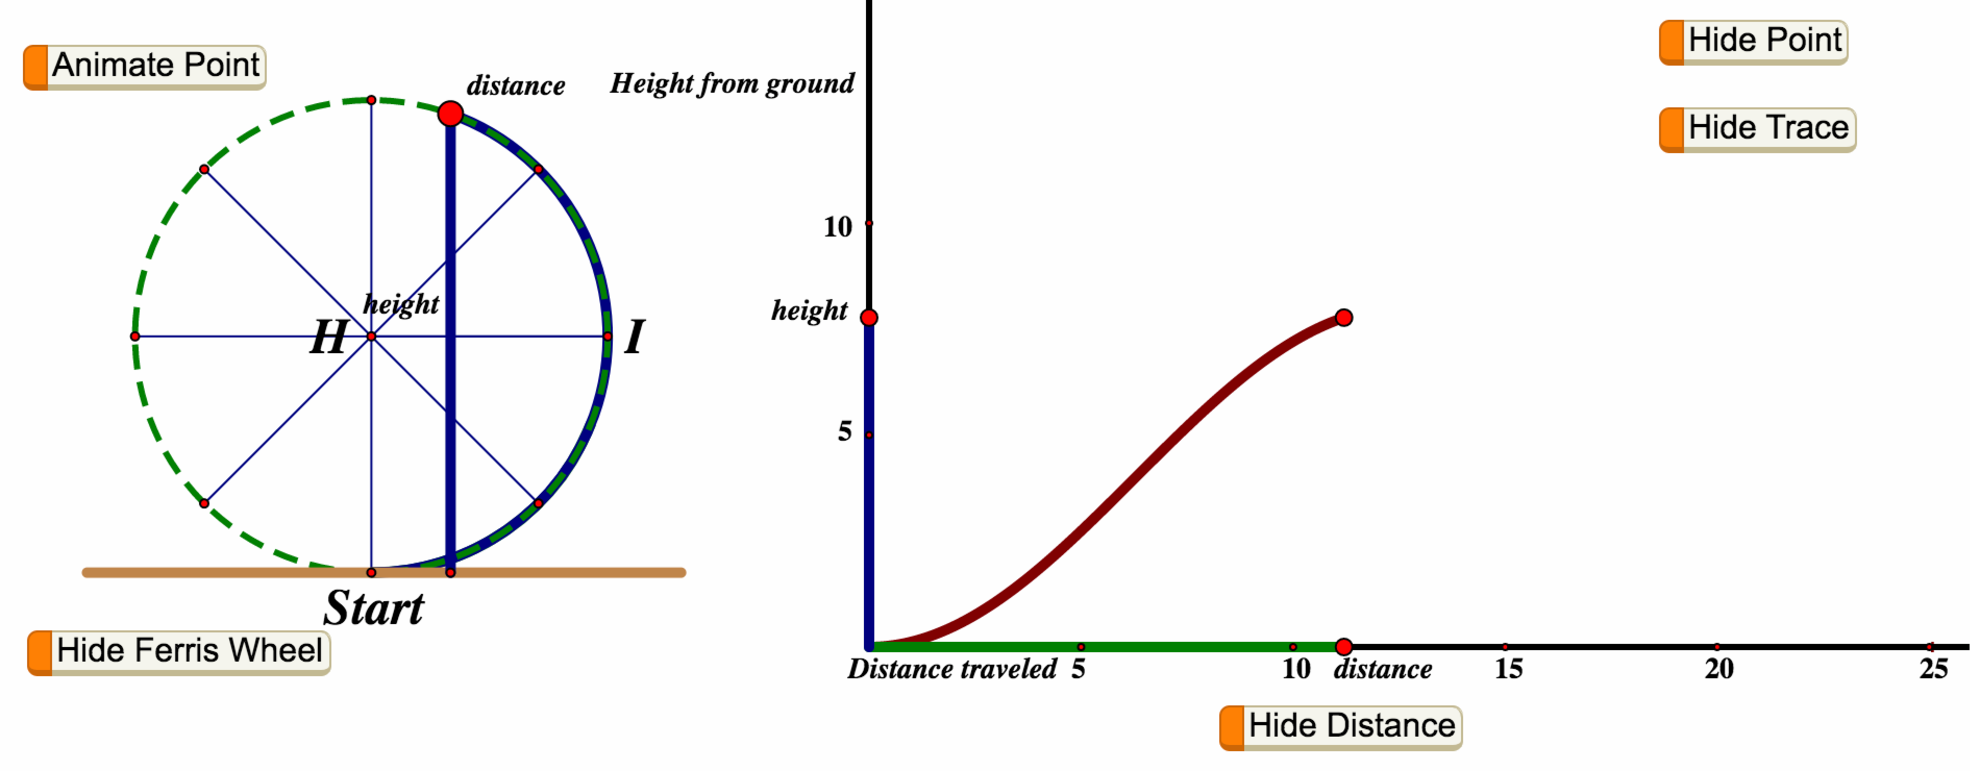
\includegraphics[width=\textwidth]{traversing-ferris-wheel-animation.pdf}
\end{image}

Because we have two quantities changing in tandem, it is natural to wonder if it is possible to represent one as a function of the other.%
\begin{exploration}
\hypertarget{p-841}{}%
In the context of the ferris wheel pictured in above, assume that the height, \(h\), of the moving point (the cab in which you are riding), and the distance, \(d\), that the point has traveled around the circumference of the ferris wheel are both measured in meters.  Further, assume that the circumference of the ferris wheel is \(150\) meters.  In addition, suppose that after getting in your cab at the lowest point on the wheel, you traverse the full circle several times.%

\begin{enumerate}[label=\alph*.]
\item
Recall that the circumference, \(C\), of a circle is connected to the circle's radius, \(r\), by the formula \(C = 2\pi r\).  What is the radius of the ferris wheel?  How high is the highest point on the ferris wheel?%
\item
How high is the cab after it has traveled \(1/4\) of the circumference of the circle?%
\item
How much distance along the circle has the cab traversed at the moment it first reaches a height of \(\frac{150}{\pi} \approx 47.75\) meters?%
\item
Can \(h\) be thought of as a function of \(d\)?  Why or why not?%
\item
Can \(d\) be thought of as a function of \(h\)?  Why or why not?%
\item
Why do you think the curve shown above has the shape that it does?  Write several sentences to explain.%
\end{enumerate}

\end{exploration}




%\typeout{************************************************}


\section{Circular Functions}

The natural phenomenon of a point moving around a circle leads to interesting relationships.  Let's consider a point traversing a circle of circumference \(24\) and examine how the point's height, \(h\), changes as the distance traversed, \(d\), changes.  Note particularly that each time the point traverses \(\frac{1}{8}\) of the circumference of the circle, it travels a distance of \(24 \cdot \frac{1}{8} = 3\) units, as seen below where each noted point lies \(3\) additional units along the circle beyond the preceding one.%

\begin{image}
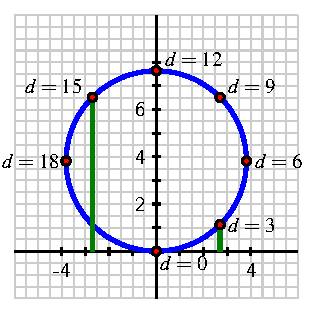
\includegraphics{traversing-first-example.pdf}
\end{image}

Note that we know the exact heights of certain points.  Since the circle has circumference \(C = 24\), we know that \(24 = 2\pi r\) and therefore \(r = \frac{12}{\pi} \approx 3.82\).  Hence, the point where \(d = 6\) (located \(1/4\) of the way along the circle) is at a height of \(h = \frac{12}{\pi} \approx 3.82\).  Doubling this value, the point where \(d = 12\) has height \(h = \frac{24}{\pi} \approx 7.64\).  Other heights, such as those that correspond to \(d = 3\) and \(d = 15\) (identified on the figure by the green line segments) are not obvious from the circle's radius, but can be estimated from the grid in the graph above as \(h \approx 1.1\) (for \(d = 3\)) and \(h \approx 6.5\) (for \(d = 15\)).  Using all of these observations along with the symmetry of the circle, we can determine the other entries in the table below.

\begin{center}
\textbf{Data for height, \(h\), as a function of distance traversed, \(d\).}
\end{center}
$$
\begin{array}{cccccccccc}
d&0&3&6&9&12&15&18&21&24\\
\hline
h&0&1.1&3.82&6.5&7.64&6.5&3.82&1.1&0
\end{array}
$$
Moreover, if we now let the point continue traversing the circle, we observe that the \(d\)-values will increase accordingly, but the \(h\)-values will repeat according to the already-established pattern, resulting in the data in the table below.

\begin{center}
\textbf{Additional data for height, \(h\), as a function of distance traversed, \(d\).}
\end{center}
$$
\begin{array}{cccccccccc}
d&24&27&30&33&36&39&42&45&48\\
\hline
h&0&1.1&3.82&6.5&7.64&6.5&3.82&1.1&0
\end{array}
$$
It is apparent that each point on the circle corresponds to one and only one height, and thus we can view the height of a point as a function of the distance the point has traversed around the circle, say \(h = f(d)\).  Using the data from the two tables and connecting the points in an intuitive way, we get the graph shown below.%

\begin{center}
The height, \(h\), of a point traversing a circle of radius \(24\) as a function of distance, \(d\), traversed around the circle.
\end{center}

\begin{image}
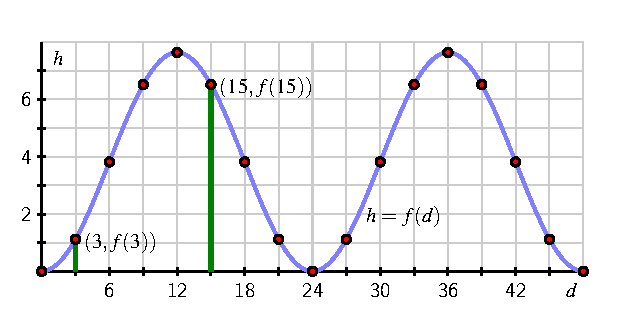
\includegraphics{traversing-first-example-graph.pdf}
\end{image}

The function \(h = f(d)\) we have been discussing is an example of what we will call a \dfn{circular function}.  Indeed, it is apparent that if we:
\begin{itemize}[label=\textbullet]
\item
take any circle in the plane,%
\item
choose a starting location for a point on the circle,%
\item
let the point traverse the circle continuously,%
\item
and track the height of the point as it traverses the circle,%
\end{itemize}
the height of the point is a function of distance traversed and the resulting graph will have the same basic shape as the curve shown in the graph above.  It also turns out that if we track the location of the \(x\)-coordinate of the point on the circle, the \(x\)-coordinate is also a function of distance traversed and its curve has a similar shape to the graph of the height of the point (the \(y\)-coordinate).  Both of these functions are circular functions because they are generated by motion around a circle.

\begin{exploration}
Consider the circle pictured below that is centered at the point \((2,2)\) and that has circumference \(8\).  Assume that we track the \(y\)-coordinate (that is, the height, \(h\)) of a point that is traversing the circle counterclockwise and that it starts at \(P_0\) as pictured.

\begin{image}
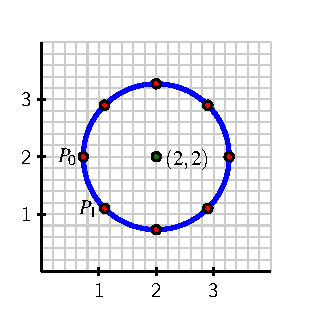
\includegraphics{traversing-act-circle.pdf}
\end{image}

\begin{enumerate}[label=\alph*.]
\item
How far along the circle is the point \(P_1\) from \(P_0\)?  Why?%
\item
Label the subsequent points in the figure \(P_2\), \(P_3\), \(\ldots\) as we move counterclockwise around the circle.  What are the exact coordinates of \(P_2\)?  of \(P_4\)?  Why?%
\item
Determine the coordinates of the remaining points on the circle (exactly where possible, otherwise approximately) and hence complete the entries in the table below that track the height, \(h\), of the point traversing the circle as a function of distance traveled, \(d\).%
%$$
%\begin{array}{cccccccccccccccccc}
%d&0&1&2&3&4&5&6&7&8&9&10&11&12&13&14&15&16\\
%\hline
%h&2$)&\(\)&\(\)&\(\)&\(\)&\(\)&\(\)&\(\)&\(\)&\(\)&\(\)&\(\)&\(\)&\(\)&\(\)&\(\)
%\end{array}
%$$
\item
By plotting the points in the table and connecting them in an intuitive way, sketch a graph of \(h\) as a function of \(d\) on the axes provided over the interval \(0 \le d \le 16\).  Clearly label the scale of your axes and the coordinates of several important points on the curve.
\begin{image}
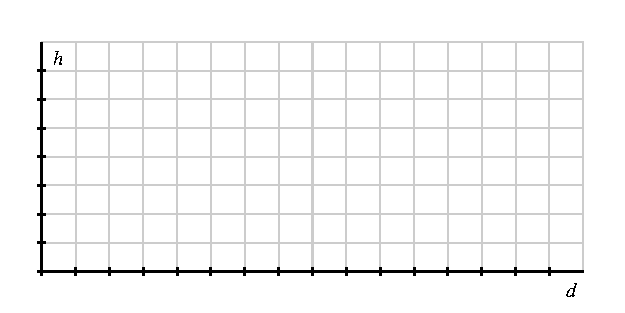
\includegraphics{traversing-act-circular-grid.pdf}
\end{image}
\item
What is similar about your graph in comparison to the one in we created at the beginning of this section?  What is different?%
\item
What will be the value of \(h\) when \(d = 51\)?  How about when \(d = 102\)?%
\end{enumerate}

\end{exploration}


%\typeout{************************************************}


\section{Properties of Circular Functions}

Every circular function has several important features that are connected to the circle that defines the function.  For the discussion that follows, we focus on circular functions that result from tracking the \(y\)-coordinate of a point traversing counterclockwise a circle of radius \(a\) centered at the point \((k,m)\).  Further, we will denote the circumference of the circle by the letter \(p\).%

\begin{image}
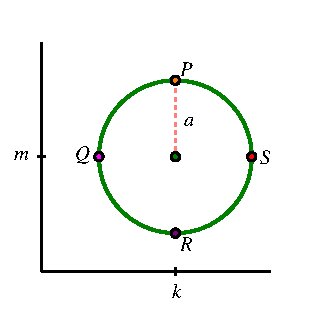
\includegraphics{traversing-circular-properties-circle.pdf}
\end{image}

We assume that the point traversing the circle starts at \(P\) in teh graph of the circle above.  Its height is initially \(y = m + a\), and then its height decreases to \(y = m\) as we traverse to \(Q\).  Continuing, the point's height falls to \(y = m - a\) at \(R\), and then rises back to \(y = m\) at \(S\), and eventually back up to \(y = m+a\) at the top of the circle.  If we plot these heights continuously as a function of distance, \(d\), traversed around the circle, we get the curve shown below. 

\begin{image}
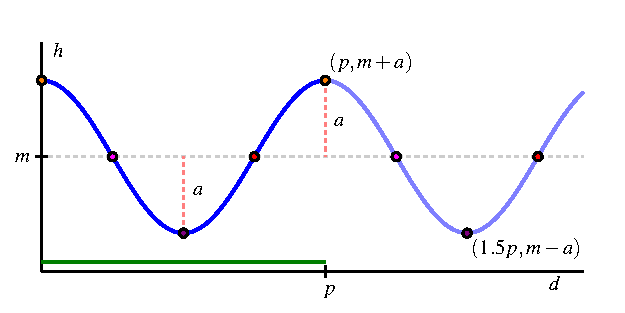
\includegraphics{traversing-circular-properties-graph.pdf}
\end{image}

This curve has several important features for which we introduce important terminology.%

\begin{definition}
The \dfn{midline} \index{circular function!midline} of a circular function is the horizontal line \(y = m\) for which half the curve lies above the line and half the curve lies below.  If the circular function results from tracking the \(y\)-coordinate of a point traversing a circle, \(y = m\) corresponds to the \(y\)-coordinate of the center of the circle.  In addition, the \dfn{amplitude} \index{circular function!amplitude} of a circular function is the maximum deviation of the curve from the midline.  Note particularly that the value of the amplitude, \(a\), corresponds to the radius of the circle that generates the curve.%

Because we can traverse the circle in either direction and for as far as we wish, the domain of any circular function is the set of all real numbers.  From our observations about the midline and amplitude, it follows that the range of a circular function \index{circular function!range} with midline \(y = m\) and amplitude \(a\) is the interval \([m-a,m+a]\).
\end{definition}

This graph is an example of a periodic function.  Recall the definition of a periodic function.

\begin{definition}
\index{function!periodic}\index{period}
Let \(f\) be a function whose domain and codomain are each the set of all real numbers.  We say that \(f\) is \dfn{periodic} provided that there exists a real number \(k\) such that \(f(x+k) = f(x)\) for every possible choice of \(x\).  The smallest value \(p\) for which \(f(x+p) = f(x)\) for every choice of \(x\) is called the \dfn{period} of \(f\).%
\end{definition}

For a circular function, the period is always the circumference of the circle that generates the curve.  In the graph of the function above, we see how the curve has completed one full cycle of behavior every \(p\) units, regardless of where we start on the curve.%

Circular functions arise as models for important phenomena in the world around us, such as in a \emph{harmonic oscillator}. \index{harmonic oscillator}  Consider a mass attached to a spring where the mass sits on a frictionless surface.  After setting the mass in motion by stretching or compressing the spring, the mass will oscillate indefinitely back and forth, and its distance from a fixed point on the surface turns out to be given by a circular function.%

%\begin{exploration}
%A weight is placed on a frictionless table next to a wall and attached to a spring that is fixed to the wall.  From its natural position of rest, the weight is imparted an initial velocity that sets it in motion.  The weight then oscillates back and forth, and we can measure its distance, \(h = f(t)\) (in inches) from the wall at any given time, \(t\) (in seconds). A graph of \(f\) and a table of select values are given below.%
%$$
%\begin{array}{cc}
%t&f(t)\\
%\hrule
%0.25&6.807\\
%0.5&4.464\\
%0.75&3.381\\
%1&3.000\\
%1.25&3.381\\
%1.5&4.464\\
%1.75&6.087\\
%2&8.000\\
%2.25&9.913\\
%2.5&11.536\\
%2.75&12.619\\
%3&13.000\\
%3.25&12.619\\
%3.5&11.536\\
%3.75&9.913\\
%4&8.000
%\end{array}
%$$
%\begin{image}
%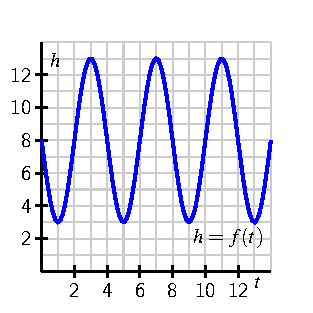
\includegraphics{traversing-circular-act-oscillator.pdf}
%\end{image}
%
%\begin{enumerate}[label=\alph*.]
%\item
%Determine the period \(p\), midline \(y = m\), and amplitude \(a\) of the function \(f\).%
%\item
%What is the furthest distance the weight is displaced from the wall?  What is the least distance the weight is displaced from the wall? What is the range of \(f\)?%
%\item
%Determine the average rate of change of \(f\) on the intervals \([4,4.25]\) and \([4.75,5]\).  Write one careful sentence to explain the meaning of each (including units).  In addition, write a sentence to compare the two different values you find and what they together say about the motion of the weight.%
%\item
%Based on the periodicity of the function, what is the value of \(f(6.75)\)? of \(d(11.25)\)?%
%\end{enumerate}
%\end{exploration}


%\typeout{************************************************}


\section{The Average Rate of Change of a Circular Function}

Just as there are important trends in the values of a circular function, there are also interesting patterns in the average rate of change of the function.  These patterns are closely tied to the geometry of the circle.%

For the next part of our discussion, we consider a circle of radius \(1\) centered at \((0,0)\), and consider a point that travels a distance \(d\) counterclockwise around the circle with its starting point viewed as \((1,0)\).  We use this circle to generate the circular function \(h = f(d)\) that tracks the height of the point at the moment the point has traversed \(d\) units around the circle from \((1,0)\).  Let's consider the average rate of change of \(f\) on several intervals that are connected to certain fractions of the circumference.%

Remembering that \(h\) is a function of distance traversed along the circle, it follows that the average rate of change of \(h\) on any interval of distance between two points \(P\) and \(Q\) on the circle is given by%
\begin{equation*}
\av_{[P,Q]} = \frac{\text{change in height}}{\text{distance along the circle}}\text{,}
\end{equation*}
where both quantities are measured from point \(P\) to point \(Q\).%


First, we consider points \(P\), \(Q\), and \(R\) where \(Q\) results from traversing \(1/8\) of the circumference from \(P\), and \(R\) \(1/8\) of the circumference from \(Q\).  In particular, we note that the distance \(d_1\) along the circle from \(P\) to \(Q\) is the same as the distance \(d_2\) along the circle from \(Q\) to \(R\), and thus \(d_1 = d_2\).  At the same time, it is apparent from the geometry of the circle that the change in height \(h_1\) from \(P\) to \(Q\) is greater than the change in height \(h_2\) from \(Q\) to \(R\), so \(h_1 \gt h_2\).  Thus, we can say that%
\begin{equation*}
\av_{[P,Q]} = \frac{h_1}{d_1} \gt \frac{h_2}{d_2} = \av_{[Q,R]} \text{.}
\end{equation*}

\begin{image}
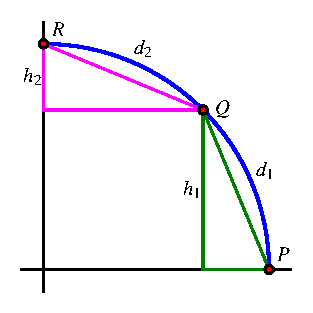
\includegraphics{traversing-circular-aroc-circle-eighth.pdf}
\end{image}

The differences in certain average rates of change appear to become more extreme if we consider shorter arcs along the circle.  Next we consider traveling \(1/20\) of the circumference along the circle.  In the graph below, points \(P\) and \(Q\) lie \(1/20\) of the circumference apart, as do \(R\) and \(S\), so here \(d_1 = d_5\).  In this situation, it is the case that \(h_1 \gt h_5\) for the same reasons as above, but we can say even more.  From the green triangle, we see that \(h_1 \approx d_1\) (while \(h_1 \lt d_1\)), so that \(\av_{[P,Q]} = \frac{h_1}{d_1} \approx 1\).  At the same time, in the magenta triangle in the figure we see that \(h_5\) is very small, especially in comparison to \(d_5\), and thus \(\av_{[R,S]} = \frac{h_5}{d_5} \approx 0\).  Hence, in this graph,%
\begin{equation*}
\av_{[P,Q]} \approx 1 \text{ and } \av_{[R,S]} \approx 0\text{.}
\end{equation*}

\begin{image}
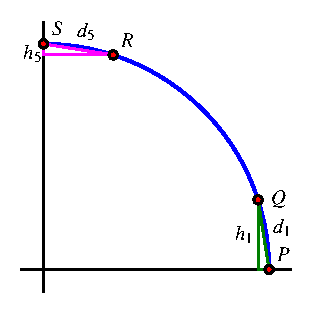
\includegraphics{traversing-circular-aroc-circle-20th.pdf}
\end{image}


This information tells us that a circular function appears to change most rapidly for points near its midline and to change least rapidly for points near its highest and lowest values.%

We can study the average rate of change not only on the circle itself, but also on a generic circular function graph, and thus make conclusions about where the function is increasing, decreasing, concave up, and concave down.%

\begin{image}
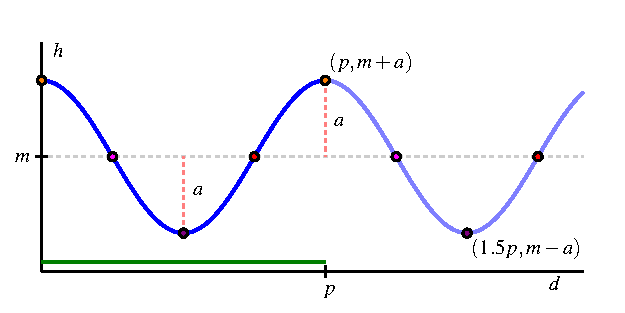
\includegraphics{traversing-circular-properties-graph.pdf}
\end{image}

%\begin{exploration}
%Consider again a weight that a oscillates back and forth on a frictionless table with distance from the wall given by, \(h = f(t)\) (in inches) at any given time, \(t\) (in seconds). A graph of \(f\) and a table of select values are given below.%
%$$
%\begin{array}{cc}
%t&f(t)\\
%\hrule
%0.25&6.807\\
%0.5&4.464\\
%0.75&3.381\\
%1&3.000\\
%1.25&3.381\\
%1.5&4.464\\
%1.75&6.087\\
%2&8.000\\
%2.25&9.913\\
%2.5&11.536\\
%2.75&12.619\\
%3&13.000\\
%3.25&12.619\\
%3.5&11.536\\
%3.75&9.913\\
%4&8.000
%\end{array}
%$$
%\begin{image}
%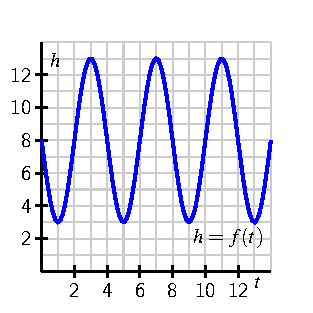
\includegraphics{traversing-circular-act-oscillator.pdf}
%\end{image}
%
%
%\begin{enumerate}[label=\alph*.]
%\item
%Determine \(\av_{[2,2.25]}\), \(\av_{[2.25,2.5]}\), \(\av_{[2.5,2.75]}\), and \(\av_{[2.75,3]}\).  What do these four values tell us about how the weight is moving on the interval \([2,3]\)?%
%\item
%Give an example of an interval of length \(0.25\) units on which \(f\) has its most negative average rate of change.  Explain your choice.%
%\item
%Give the largest example you can of an interval on which \(f\) is decreasing.%
%\item
%Give an example of an interval on which \(f\) is concave up.\footnote{Recall that a function is concave up on an interval provided that throughout the interval, the curve bends upward, similar to a parabola that opens up.\label{fn-23}}%
%\item
%On an interval where \(f\) is both decreasing and concave down, what does this tell us about how the weight is moving on that interval?  For instance, is the weight moving toward or away from the wall?  is it speeding up or slowing down?%
%\item
%What general conclusions can you make about the average rate of change of a circular function on intervals near its highest or lowest points?  about its average rate of change on intervals near the function's midline?%
%\end{enumerate}
%%
%\end{exploration}

\begin{summary}\begin{itemize}
\item When a point traverses a circle, a corresponding function can be generated by tracking the height of the point as it moves around the circle, where height is viewed as a function of distance traveled around the circle.  We call such a function a \emph{circular function}.  
%\begin{image}
%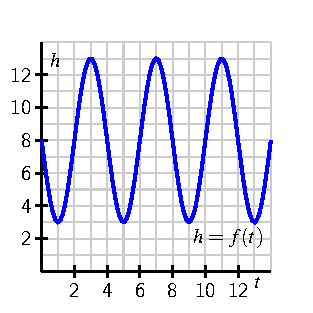
\includegraphics{traversing-circular-act-oscillator.pdf}
%\end{image}
\item Circular functions have several standard features.  The function has a \emph{midline} that is the line for which half the points on the curve lie above the line and half the points on the curve lie below.  A circular function's \emph{amplitude} is the maximum deviation of the function value from the midline; the amplitude corresponds to the radius of the circle that generates the function.  Circular functions also repeat themselves, and we call the smallest value of \(p\) for which \(f(x+p) = f(x)\) for all \(x\) the period of the function.  The period of a circular function corresponds to the circumference of the circle that generates the function.%
\item Non-constant linear functions are either always increasing or always decreasing; quadratic functions are either always concave up or always concave down.  Circular functions are sometimes increasing and sometimes decreasing, plus sometimes concave up and sometimes concave down.  These behaviors are closely tied to the geometry of the circle.%
\end{itemize}\end{summary}

\end{document}
